\documentclass[conference]{IEEEtran}
\IEEEoverridecommandlockouts
% The preceding line is only needed to identify funding in the first footnote. If that is unneeded, please comment it out.
\usepackage{cite}
\usepackage{amsmath,amssymb,amsfonts}

\usepackage{graphicx}
\usepackage{textcomp}
\usepackage{xcolor}
\def\BibTeX{{\rm B\kern-.05em{\sc i\kern-.025em b}\kern-.08em
    T\kern-.1667em\lower.7ex\hbox{E}\kern-.125emX}}
\begin{document}

\title{Blockchain Technology

\thanks{Identify applicable funding agency here. If none, delete this.}
}


\author{\IEEEauthorblockN{Sohel S. Bargir}
\IEEEauthorblockA{\textit{Computer Engineering} \\
\textit{COEP Technological University}\\
Pune, India \\
sohelbargir2@gmail.com}
}

\maketitle

\begin{abstract}
Blockchain, the foundation of Bitcoin, has received
extensive attentions recently. Blockchain serves as an immutable
ledger which allows transactions take place in a decentralized
manner. Blockchain-based applications are springing up, cov-
ering numerous fields including financial services, reputation
system and Internet of Things (IoT), and so on. However,
there are still many challenges of blockchain technology such
as scalability and security problems waiting to be overcome.
This paper presents a comprehensive overview on blockchain
technology. We provide an overview of blockchain architechture
firstly and compare some typical consensus algorithms used
in different blockchains. Furthermore, technical challenges and
recent advances are briefly listed. We also lay out possible future
trends for blockchain.
\end{abstract}

\begin{IEEEkeywords}
Blockchain, decentralization, consensus, scala-
bility
\end{IEEEkeywords}

\section{Introduction}
Nowadays cryptocurrency has become a buzzword in both
industry and academia. As one of the most successful cryp-
tocurrency, Bitcoin has enjoyed a huge success with its capital
market reaching 10 billion dollars in 2016 [1]. With a spe-
cially designed data storage structure, transactions in Bitcoin
network could happen without any third party and the core
technology to build Bitcoin is blockchain, which was first
proposed in 2008 and implemented in 2009 [2]. Blockchain
could be regarded as a public ledger and all committed
transactions are stored in a list of blocks. This chain grows
as new blocks are appended to it continuously. Asymmetric
cryptography and distributed consensus algorithms have been
implemented for user security and ledger consistency. The
blockchain technology generally has key characteristics of
decentralization, persistency, anonymity and auditability. With
these traits, blockchain can greatly save the cost and improve
the efficiency.
Since it allows payment to be finished without any bank or
any intermediary, blockchain can be used in various financial
services such as digital assets, remittance and online payment
[3], [4]. Additionally, it can also be applied into other fields
including smart contracts [5], public services [6], Internet of
Things (IoT) [7], reputation systems [8] and security services
[9]. Those fields favor blockchain in multiple ways. First of all,
blockchain is immutable. Transaction cannot be tampered once
it is packed into the blockchain. Businesses that require high
reliability and honesty can use blockchain to attract customers.
Besides, blockchain is distributed and can avoid the single
point of failure situation. As for smart contracts, the contract
could be executed by miners automatically once the contract
has been deployed on the blockchain.
Although the blockchain technology has great potential for
the construction of the future Internet systems, it is facing a
number of technical challenges. Firstly, scalability is a huge
concern. Bitcoin block size is limited to 1 MB now while
a block is mined about every ten minutes. Subsequently, the
Bitcoin network is restricted to a rate of 7 transactions per
second, which is incapable of dealing with high frequency
trading. However, larger blocks means larger storage space
and slower propagation in the network. This will lead to
centralization gradually as less users would like to maintain
such a large blockchain. Therefore the tradeoff between block
size and security has been a tough challenge. Secondly, it has
been proved that miners could achieve larger revenue than
their fair share through selfish mining strategy [10]. Miners
hide their mined blocks for more revenue in the future. In
that way, branches could take place frequently, which hinders
blockchain development. Hence some solutions need to be put
forward to fix this problem. Moreover, it has been shown that
privacy leakage could also happen in blockchain even users
only make transactions with their public key and private key
[11]. Furthermore, current consensus algorithms like proof of
work or proof of stake are facing some serious problems. For
example, proof of work wastes too much electricity energy
while the phenomenon that the rich get richer could appear in
the proof of stake consensus process.
There is a lot of literature on blockchain from various
sources, such as blogs, wikis, forum posts, codes, confer-
ence proceedings and journal articles. Tschorsch et al. [12]
made a technical survey about decentralized digital currencies
2017 IEEE 6th International Congress on Big Data
978-1-5386-1996-4/17 31.00 © 2017 IEEE
DOI 10.1109/BigDataCongress.2017.85
557
including Bitcoin. Compared to [12], our paper focuses on
blockchain technology instead of digital currencies. Nomura
Research Institut made a technical report about blockchain
[13]. Contrast to [13], our paper focuses on state-of-art
blockchain researches including recent advances and future
trends.
The rest of this paper is organized as follows. Section II
introduces blockchain architecture. Section III shows typical
consensus algorithms used in blockchain. Section IV summa-
rizes the technical challenges and the recent advances in this
area. Section V discusses some possible future directions and
section VI concludes the paper 

\section{Blockchain Architecture}
Blockchain is a sequence of blocks, which holds a complete
list of transaction records like conventional public ledger
[14]. Figure 1 illustrates an example of a blockchain. With
a previous block hash contained in the block header, a block
has only one parent block. It is worth noting that uncle blocks
(children of the block’s ancestors) hashes would also be stored
in ethereum blockchain [15]. The first block of a blockchain
is called genesis block which has no parent block. We then
explain the internals of blockchain in details.

\begin{figure}
  \centering
  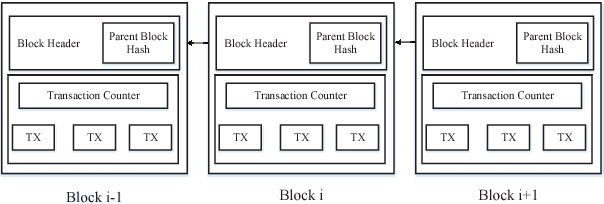
\includegraphics[scale=0.4]{fig.png}
  \caption{Some figure}
\end{figure}

\subsection{Block}

A block consists of the block header and the block body as
shown in Figure 2. In particular, the block header includes:
(i) Block version: indicates which set of block validation
rules to follow.
(ii) Merkle tree root hash: the hash value of all the transac-
tions in the block.
(iii) Timestamp: current time as seconds in universal time
since January 1, 1970.
(iv) nBits: target threshold of a valid block hash.
(v) Nonce: an 4-byte field, which usually starts with 0
and increases for every hash calculation (will be explained
in details in Section III).
(vi) Parent block hash: a 256-bit hash value that points to
the previous block.
The block body is composed of a transaction counter and
transactions. The maximum number of transactions that a
block can contain depends on the block size and the size of
each transaction. Blockchain uses an asymmetric cryptography
mechanism to validate the authentication of transactions [13].
Digital signature based on asymmetric cryptography is used in
an untrustworthy environment. We next briefly illustrate digital
signature.


\subsection{Digital Signature}

Each user owns a pair of private key and public key.
The private key that shall be kept in confidentiality is used
to sign the transactions. The digital signed transactions are
broadcasted throughout the whole network. The typical digital
signature is involved with two phases: signing phase and
verification phase. For instance, an user Alice wants to send
another user Bob a message. (1) In the signing phase, Alice
encrypts her data with her private key and sends Bob the
encrypted result and original data. (2) In the verification phase,
Bob validates the value with Alice’s public key. In that way,
Bob could easily check if the data has been tampered or not.
The typical digital signature algorithm used in blockchains is
the elliptic curve digital signature algorithm (ECDSA) [16]


\subsection{Key characterstics of Blockchain}
In summary, blockchain has following key characteristics.
• Decentralization. In conventional centralized transaction
systems, each transaction needs to be validated through
the central trusted agency (e.g., the central bank), in-
evitably resulting to the cost and the performance bottle-
necks at the central servers. Contrast to the centralized
mode, third party is no longer needed in blockchain.
Consensus algorithms in blockchain are used to maintain
data consistency in distributed network.
• Persistency. Transactions can be validated quickly and
invalid transactions would not be admitted by honest
miners. It is nearly impossible to delete or rollback
transactions once they are included in the blockchain.
Blocks that contain invalid transactions could be discov-
ered immediately.
• Anonymity. Each user can interact with the blockchain
with a generated address, which does not reveal the
real identity of the user. Note that blockchain cannot
guarantee the perfect privacy preservation due to the
intrinsic constraint (details will be discussed in section
IV)
• Auditability. Bitcoin blockchain stores data about user
balances based on the Unspent Transaction Output (UTX-
O) model [2]: Any transaction has to refer to some previ-
ous unspent transactions. Once the current transaction is
recorded into the blockchain, the state of those referred
unspent transactions switch from unspent to spent. So
transactions could be easily verified and tracked.

\subsection{Taxonomy of a blockchain systems}

Current blockchain systems are categorized roughly into
three types: public blockchain, private blockchain and con-
sortium blockchain [17]. In public blockchain, all records are
visible to the public and everyone could take part in the con-
sensus process. Differently, only a group of pre-selected nodes
would participate in the consensus process of a consortium
blockchain. As for private blockchain, only those nodes that
come from one specific organization would be allowed to join
the consensus process.
A private blockchain is regarded as a centralized network
since it is fully controlled by one organization. The consortium
blockchain constructed by several organizations is partially
decentralized since only a small portion of nodes would be
selected to determine the consensus. The comparison among
the three types of blockchains is listed in Table I.
• Consensus determination. In public blockchain, each n-
ode could take part in the consensus process. And only
a selected set of nodes are responsible for validating the
block in consortium blockchain. As for private chain, it is
fully controlled by one organization and the organization
could determine the final consensus.
• Read permission. Transactions in a public blockchain are
visible to the public while it depends when it comes to a
private blockchain or a consortium blockchain.
• Immutability. Since records are stored on a large number
of participants, it is nearly impossible to tamper trans-
actions in a public blockchain. Differently, transactions
in a private blockchain or a consortium blockchain could
be tampered easily as there are only limited number of
participants.
• Efficiency. It takes plenty of time to propagate transac-
tions and blocks as there are a large number of nodes
on public blockchain network. As a result, transaction
throughput is limited and the latency is high. With fewer
validators, consortium blockchain and private blockchain
could be more efficient.
• Centralized. The main difference among the three types
of blockchains is that public blockchain is decentralized,
consortium blockchain is partially centralized and private
blockchain is fully centralized as it is controlled by a
single group.
• Consensus process. Everyone in the world could join
the consensus process of the public blockchain. Different
from public blockchain, both consortium blockchain and
private blockchain are permissioned.
Since public blockchain is open to the world, it can at-
tract many users and communities are active. Many public
blockchains emerge day by day. As for consortium blockchain,
it could be applied into many business applications. Cur-
rently Hyperledger [18] is developing business consortium
blockchain frameworks. Ethereum also has provided tools for
building consortium blockchains [19].


\section{Conclusion}
Blockchain has shown its potential for transforming tradi-
tional industry with its key characteristics: decentralization,
persistency, anonymity and auditability. In this paper, we
present a comprehensive overview on blockchain. We first give
an overview of blockchain technologies including blockchain
architecture and key characteristics of blockchain. We then dis-
cuss the typical consensus algorithms used in blockchain. We
analyzed and compared these protocols in different respects.
Furthermore, we listed some challenges and problems that
would hinder blockchain development and summarized some
existing approaches for solving these problems. Some possible
future directions are also proposed. Nowadays blockchain-
based applications are springing up and we plan to conduct
in-depth investigations on blockchain-based applications in the
future.

\section*{Acknowledgment}

The work described in this paper was supported by the
National Key Research and Development Program (2016YF-
B1000101), the National Natural Science Foundation of China
under (61472338), the Fundamental Research Funds for the
Central Universities and Macao Science and Technology De-
velopment Fund under Grant No. 096/2013/A3. The authors
would like to thank Gordon K.-T. Hon for his constructive
comments.


\begin{thebibliography}{00}
\bibitem{b1} “State of blockchain q1 2016: Blockchain funding overtakes
bitcoin,” 2016. [Online]. Available: http://www.coindesk.com/
state-of-blockchain-q1-2016.
\bibitem{b2} S. Nakamoto, “Bitcoin: A peer-to-peer electronic cash system,” 2008.
[Online]. Available: https://bitcoin.org/bitcoin.pdf.
\bibitem{b3} G. W. Peters, E. Panayi, and A. Chapelle, “Trends in crypto-currencies
and blockchain technologies: A monetary theory and regulation
perspective,” 2015. [Online]. Available: http://dx.doi.org/10.2139/ssrn.
2646618.
\bibitem{b4} A. Kosba, A. Miller, E. Shi, Z. Wen, and C. Papamanthou, “Hawk:
The blockchain model of cryptography and privacy-preserving smart
contracts,” in Proceedings of IEEE Symposium on Security and Privacy
(SP), San Jose, CA, USA, 2016, pp. 839–858.
\bibitem{b5} G. Foroglou and A.-L. Tsilidou, “Further applications of the blockchain,”
2015.
\bibitem{b6} Y. M. Sharples and J. Domingue, “The blockchain and kudos: A distributed
system for educational record, reputation and reward,” in Proceedings of
11th European Conference on Technology Enhanced Learning (EC-TEL
2015), Lyon, France, 2015, pp. 490–496.
\bibitem{b7} . Buterin, “On public and private blockchains,”
2015. [Online]. Available: https://blog.ethereum.org/2015/08/07/
on-public-and-private-blockchains/.
\end{thebibliography}
\vspace{12pt}


\end{document}